\section{Introduction}


This project aims to use deep learning on images of food dishes. Food images are unique: there are multiple cuisines around the world; food items have unique color, size, shape and texture; and food items can be combined in several ways to prepare a meal. Using artificial intelligence on food images has the potential to revolutionize the field of dining, promote healthy eating, prevent food waste etc.

To that end, we are working on the problem of classifying food dishes. We formulate this problem as a classification task with one class per image, i.e given an image of a food dish, we want to correctly predict what dish it is. Figure~\ref{fig:imgsburgerpizza} shows sample images of two popular food categories. Being able to accurately predict a food category from an image could be useful for several application scenarios, such as knowing the calorie count for that food item, identifying its ingredients etc.  

The remainder of the paper is organized as follows. In Section~\ref{sec:relatedwork} we survey related work in the area of image classification. In Section~\ref{sec:methods} we introduce the key components used in image classification tasks. In Section~\ref{sec:datasetandfeatures} we provide details about our dataset. Section~\ref{sec:evaluationresults}  presents the experimental results from our modeling techniques. Finally, we present our conclusions in Section~\ref{sec:conclusion}.

\begin{figure}[ht!]
    \centering
    \begin{subfigure}{.4\linewidth}
        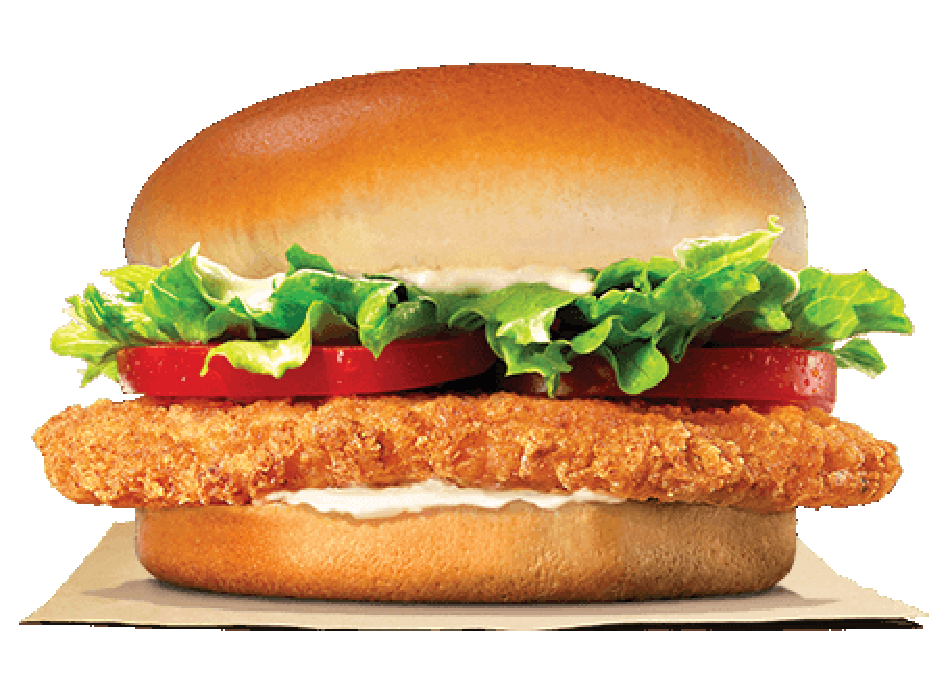
\includegraphics[height=1.25in, width=1.6in]{Figs4Paper/_final/img_burger.eps}
        \caption{burger}
    \end{subfigure}
    \hskip2em
    \begin{subfigure}{.4\linewidth}
        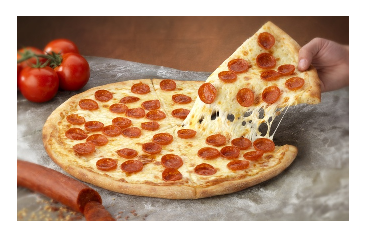
\includegraphics[height=1.25in, width=1.6in]{Figs4Paper/_final/img_pizza.eps}
        \caption{pizza}
    \end{subfigure}
    \caption{Sample images in our dataset}
		\label{fig:imgsburgerpizza}
\end{figure}

%-------------------------------------------------------------------------
